% !TeX root = ../../main.tex
\begingroup
\ChSevenBegin
\emergencystretch=2em
\chapter{Forecasting Clinical Risk from Textual Time Series: Structuring Narratives for Temporal AI in Healthcare}\label{chap:ch07}
\noindent\emph{This chapter is based on:} \cite{noroozizadeh2026forecasting}.\par\smallskip

% % !TeX root = ../../../main.tex
\begin{ChSevenAbstract}
Clinical case reports encode temporal patient trajectories that are often underexploited by traditional machine learning methods relying on structured data. 
In this work, we introduce the forecasting problem from textual time series, where timestamped clinical findings---extracted via an LLM-assisted annotation pipeline---serve as the primary input for prediction. 
We systematically evaluate a diverse suite of models, including fine-tuned decoder-based large language models and encoder-based transformers, on tasks of event occurrence prediction, temporal ordering, and survival analysis. 
Our experiments reveal that encoder-based models consistently achieve higher F1 scores and superior temporal concordance for short- and long-horizon event forecasting, while fine-tuned masking approaches enhance ranking performance. 
In contrast, instruction-tuned decoder models demonstrate a relative advantage in survival analysis, especially in early prognosis settings. 
Our sensitivity analyses further demonstrate the importance of time ordering, which requires clinical time series construction, as compared to text ordering, the format of the text inputs that LLMs are classically trained on. 
This highlights the additional benefit that can be ascertained from time-ordered corpora, with implications for temporal tasks in the era of widespread LLM use. 
\end{ChSevenAbstract}
% !TeX root = ../../../main.tex
\subsection{Sepsis-Specific Reconstruction Study}
\label{ch06:sec:intro}

The Third International Consensus Definitions for Sepsis (Sepsis-3) are the benchmark definitions for sepsis, the dysfunctional immune response to an infection, which are used in trial eligibility criteria \citep{kyriazopoulou2021procalcitonin} and phenotyping studies \citep{ch06:seymour2019derivation}.
In the critical care literature, sepsis is seen as a heterogeneous disease, a pathway arrived upon from a multitude of infectious origins, anatomical sites, and comorbid profiles.  
There is increasing recognition of the importance of time in understanding sepsis and sepsis progression, as seen in early-warning systems \citep{henry2022factors}, variation in prediction utility \citep{kamran2024evaluation}, and endotype characterization \citep{ch06:noroozizadeh2023temporal}.

Meanwhile, structured data streams, which are the data resources these tools use, are often incomplete records with insufficient information to render or confirm a diagnosis of sepsis \citep{moldwin2021empirical}. %
A more complete alternative is the discharge summary, or more generally, the case report, in which a clinician documents the clinical findings pertinent to the case and care management.
The impracticality of using the case report is that it is only written in full after the encounter is over, \emph{i.e.}, with a less granular timestamp than the events contained within. 
In principle, having a more complete, fine-grained temporal record could enable better temporal analyses of patients with sepsis, leading to better understanding and treatment improvements.

At present, the (semi-)public critical care repositories at the research frontier contain high resolution structured signals and low resolution textual signals. 
While several concerted efforts have focused on extracting temporal information, they have largely focused on temporal relations between clinical concepts \citep{sun2013evaluating} rather than on event timing.  
Those that have focused on timing \citep{leeuwenberg2020towards,ch06:frattallone2024using} used excerpted summaries and relatively small sample sizes. 


In order to train sepsis models that can incorporate information referenced in free text with finer temporal granularity, we seek to generate larger samples of textual time series.
To do so, we introduce a novel Sepsis-3 textual time series corpus from the PubMed Open Access (PMOA) Subset.
We adopt an LLM-as-annotator approach, evaluating both the ability of models to extract clinical findings and their ability to associate those findings with timestamps.
We augment existing clinical annotations with our own PMOA annotations and contrast LLM annotations with both our clinician annotations and the annotations of \cite{ch06:frattallone2024using}.
Because the corpus is automatically generated beyond the manually annotated subset, we validate it through a multi-layer framework: clinician-annotated gold-standard evaluation on \texttt{sepsis-40}, clinician--clinician agreement, bootstrap uncertainty quantification, bronze-standard proxy-reference evaluation on \texttt{sepsis-100}, direct hallucination auditing, multi-pass self-consistency, and full-corpus cross-model agreement.
These assessments provide evidence for the quality and limitations of the LLM annotations and support the use of T2S2 as a retrospective research resource for temporal modeling of sepsis trajectories.

% !TeX root = ../../../main.tex
\begin{sloppypar}
\subsubsection{Related work}
Numerous critical care and sepsis datasets are available \mbox{(semi-)publicly}, \emph{e.g.}, \cite{thoral2021sharing,pollard2018eicu}, including several with de-identified clinical discharge summaries: MIMIC-III \citep{ch06:johnson2016mimic}
and MIMIC-IV \citep{ch06:johnson2023mimic}. 
Sepsis phenotyping (including Sepsis-3) has been conducted using a variety of methods on structured data \citep{johnson2018comparative}, although structured data is often highly missing, leading to suboptimal phenotyping \citep{seinen2025using}.
Additionally, the timing of sepsis phenotyping is crucial, in that delays in sepsis prediction can nullify predictiveness and lead to burdensome and unhelpful analytic models \citep{kamran2024evaluation}.  
\end{sloppypar}

Several works have used the i2b2 (a competition subset of MIMIC-II/III) to construct timelines of clinical concepts \citep{leeuwenberg2020towards,ch06:frattallone2024using}.  
In the case of \cite{leeuwenberg2020towards}, the event spans are already given, and focus on an excerpt of the full discharge summary, so we focus our direct comparison on that of \cite{ch06:frattallone2024using}.
In contrast to these works, we adopt an annotation process focused on temporal assignment to clinical findings rather than i2b2 clinical concepts \citep{ch06:uzuner20112010}, which allows for greater specificity of the event in the absence of additional context.  
Additionally, as compared to \cite{ch06:frattallone2024using},
we focus on using text alone for clinical time series construction, which is necessary for the PubMed Open Access Subset since no complementary data source is available.

Broadly in the medical domain, LLMs are showing promise in medical tasks such as summarization \citep{van2024adapted}.
In fact, some findings suggest that 
medical fine-tuning rarely leads to improved performance over the corresponding foundation models \citep{jeong-etal-2024-medical}. 
In our analysis, we primarily use foundation LLMs and show that their scale and instruction-tuning are central to the performance of the model.  


% !TeX root = ../../../main.tex
\subsection{Methods}

We next describe our forecasting data and annotation provenance, define the forecasting and survival prediction tasks, detail the modeling approaches evaluated, and present the sensitivity analyses used to assess robustness (Figure~\ref{ch07:fig:flowchart}). \footnote{Our code can be found at: \url{https://github.com/Shahriarnz14/Textual-Time-Series-Forecasting}.
% \\
% \hspace*{1.8em}The extended version of this paper, including the full technical appendix, is available in \citet{ch07:noroozizadeh2025forecasting}.
}


% !TeX root = ../../../main.tex
\begin{figure}[htbp]
\begin{ChSevenFloatBody}
\centering
    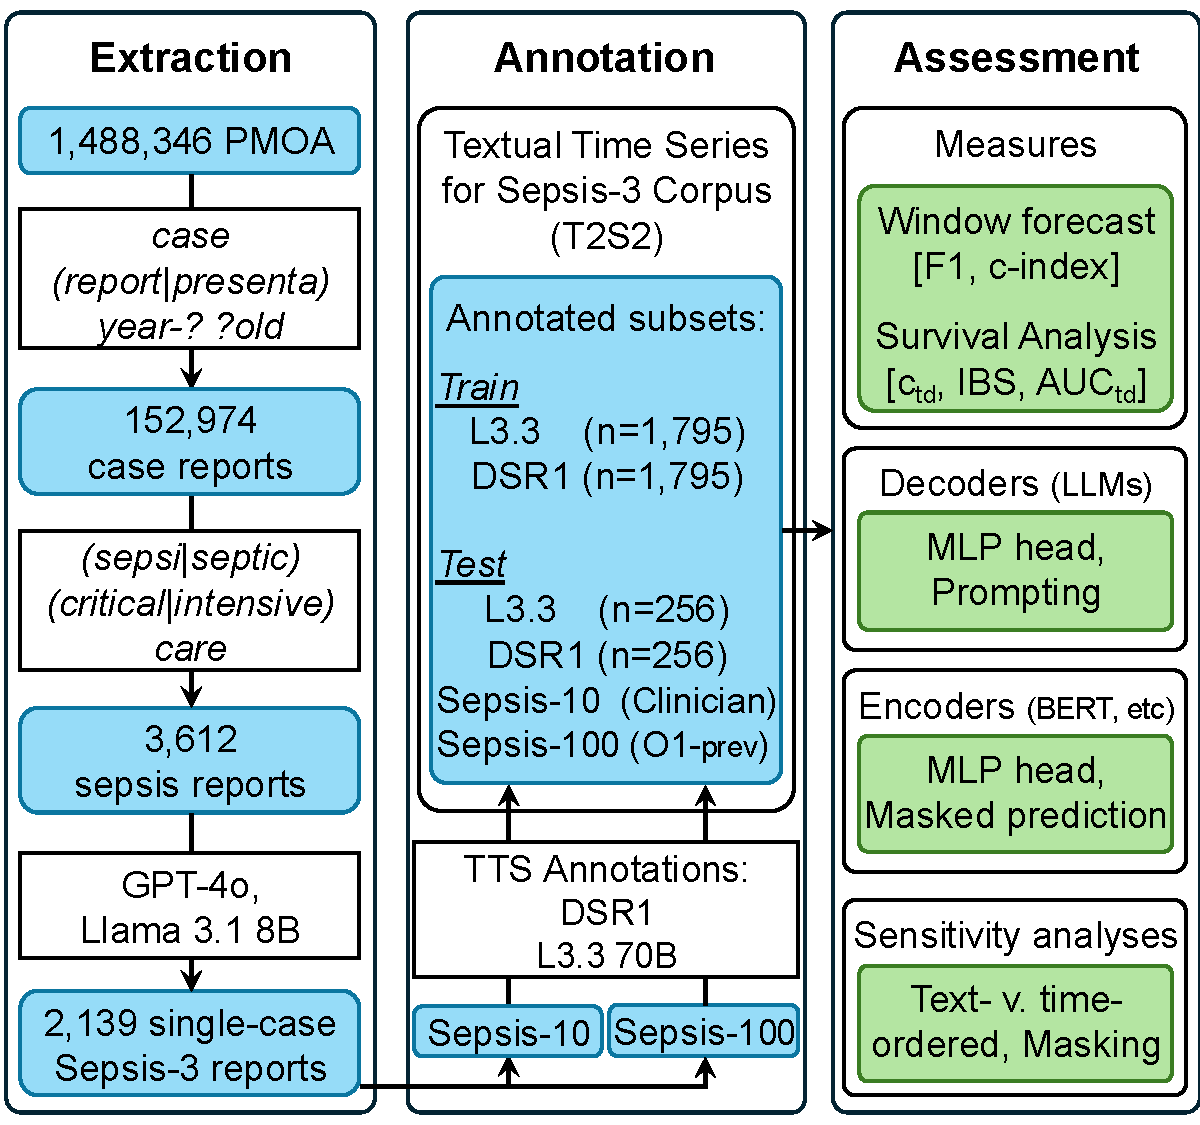
\includegraphics[width=\linewidth]{Chapters/chapter-06/images/Figures/ttsforecast_flowchart_updated.pdf}
    
    

\end{ChSevenFloatBody}
\caption{\textit{T2S2} forecasting analysis pipeline}\ChSevenFloatLabel{ch07:fig:flowchart}
\end{figure}



% !TeX root = ../../../main.tex
\subsubsection{Forecasting Corpus}
We used the PubMed Open Access (PMOA) Subset (as of December 17, 2024) for our analysis.
The case-report extraction and Sepsis-3 screening pipeline is described in Chapter~\ref{chap:ch05}.
This multi-step process yielded a total of 2,139 Sepsis-3 case reports.
\par

% !TeX root = ../../../main.tex
\subsubsection{Textual Time Series Annotation}
\label{ch07:sec:tts-annotation}

Following \citet{ch07:noroozizadeh2025reconstructing}, a textual time series case report corpus of Sepsis-3 patients was constructed from the PMOA sepsis reports.

We used \texttt{DeepSeek-R1-UD-IQ1} and \texttt{Llama-3.3-70B-Instruct} models to generate clinical textual time series from the 2,139 sepsis case reports.
We refer to this as \textbf{T}extual \textbf{T}ime-\textbf{S}eries for \textbf{S}epsis (\textit{T2S2}).
The shared reconstruction methodology and extraction prompts are provided in Chapter~\ref{chap:ch05} and Appendix~\ref{app:ch05}.
Our dataset was split into development (n = 1,795; 80\% train, 20\% validation), testing \textit{T2S2}-test (n = 244), and 100 historical reference reports comprising \textit{sepsis-10} (n = 10; clinician-annotated) and \textit{sepsis-100} (n = 90; \texttt{O1-preview}-annotated).
These historical forecasting annotations and reference sets are distinct from the newer reconstruction evaluation in Chapter~\ref{chap:ch05}.
\par

% !TeX root = ../../../main.tex
\subsubsection{Prediction-Instance Construction}\label{ch07:sec:prediction-instances}

We develop a general framework for predictive modeling over textual time series of the encoder-only models, designed to accommodate the irregular, event-based structure common to clinical case reports. 
As highlighted Section~\ref{ch07:sec:tts-annotation}, each data instance consists of a sequence of clinical events, where each event is a free-text string describing a clinical finding, intervention, or diagnosis, paired with a timestamp in hours relative to the time of admission. 
The format resembles a two-column table, where the first column contains textual clinical events and the second column contains integer-valued timestamps.

\ChSevenParagraph{Input Preprocessing and Timeseries Construction.}
From each case report, we construct multiple training examples for sequence forecasting.
For a fixed number $K$ of candidate future events, we generate overlapping windows of historical events and forecast targets.
Specifically, for each case report with $L$ rows, we construct a sequence of up to $L-K$ forecasting examples.
Each example is structured as follows:

\begin{itemize}
    \item A \textbf{history segment} $\mathcal{H}_t = \{(e_i, t_i)\}_{i=1}^{n}$, consisting of clinical events $e_i$ occurring at timestamps $t_i \leq t$.
    \item A \textbf{forecast target} $\mathcal{F}_t = \{(f_j, \tau_j)\}_{j=1}^{K}$, consisting of the next $K$ events after $t$.
\end{itemize}

To preserve the temporal coherence of events, we treat all events with the same timestamp as an atomic unit.
That is, if multiple events share the same timestamp, they are included together in the history or forecast block, and the next forecasting window is only advanced after the full timestamp block has been consumed.

\ChSevenParagraph{Model Input Representation.}
Each training example is serialized into a transformer-compatible input by linearizing the historical events and forecast events.
Importantly, we preserve both temporal and textual content by encoding each historical event in the form ``\texttt{t:e}'' where \texttt{t} is the timestamp and \texttt{e} is the event string.
The input to the language model takes the form:

\begin{equation}
\texttt{[CLS]} \; t_1\texttt{:}e_1 \; \texttt{[SEP]} \; t_2\texttt{:}e_2 \; \texttt{[SEP]} \; \dots \; \texttt{[SEP]} \; t_n\texttt{:}e_n
\end{equation}

All inputs are truncated from the left (i.e., keeping the most recent tokens) if they exceed the model's context window (typically 512 tokens).

Target-specific input components are described in Appendix~\ref{ch07:apd:encoder-forecasting}.
\par

% !TeX root = ../../../main.tex
\subsubsection{Forecasting Tasks}
Using the timelines extracted from the annotations, we defined two primary forecasting tasks and a survival analysis task as follows:

\ChSevenParagraph{Event Occurrence Prediction.} 
Given a prefix of the clinical timeline (all events up to a certain time $t$), the model is tasked with predicting whether each of the immediate next $k$ events occurs within a specified time horizon. 
This setup is repeated across multiple time cut-offs to simulate an “online” forecasting scenario, where the model must output a binary label for each of the next $k$ events:
does this event occur within $h$ hours after $t$? 
Time horizons used include 1 hour, 24 hours (1 day), and 168 hours (1 week). 
The task is framed as a series of binary classification problems, with one binary decision per event. 
Evaluation is based on precision, recall, and macro-F1 across classes for each time horizon.

\ChSevenParagraph{Temporal Ordering Prediction.} 
This task assesses the model's ability to reconstruct the correct sequence of future events. 
At each time cut-off $t$, we extract the next $k$ events from the timeline and remove their timestamps. 
The model must output a permutation of these events that matches their true chronological order.
This is framed as a ranking task, evaluated by computing the pairwise concordance between the predicted and true orderings (e.g., proportion of correctly ordered pairs). 
This tests whether the model can infer temporal progression from unordered event content alone.

\ChSevenParagraph{Survival Analysis for Mortality Time.}  
We include a classical survival analysis task to model time until death. 
Many case reports specify whether the patient died and, if so, when (e.g., "the patient died on hospital day 10"), which enables us to define a time-to-event outcome. 
For this task, we evaluate models at predefined cut-off times--- specifically at 0 hours (admission), 24 hours (1 day), and 168 hours (1 week)--- and use the extracted event history up to each cut-off as input. 
A survival model is trained to predict the probability of survival over time beyond each cut-off. 
We evaluate using the time-dependent concordance to measure alignment of the predicted survival times with actual outcomes.


% !TeX root = ../../../main.tex
\subsubsection{Modeling Approaches}
To evaluate performance on the event forecasting and survival prediction tasks, we implement five modeling paradigms: (i) decoder-only large language models (LLMs) with fine-tuned heads, (ii) prompted LLMs without gradient updates (zero- or few-shot), (iii) encoder-only models with task-specific fine-tuned heads, (iv) encoder-masking models with fine-tuning, and (v) encoder-masking models in zero-shot settings.
In Appendix~\ref{ch07:apd:encoder-forecasting} and~\ref{ch07:apd:encoder-survival}, we provide technical details of encoder-based forecasting methods and survival model training respectively.

\ChSevenParagraph{(i) Fine-tuned LLMs.}  
We apply instruction-tuned decoder-only models from the \textit{Llama} and \textit{DeepSeek} families: \textit{Llama-3.3-70B-Instruct}, \textit{Llama-3.1-8B-Instruct}, and their distilled variants \citep{grattafiori2024llama,liu2024deepseek}.
We also include open-source models with documented training corpora (\textit{OLMO-32B-Instruct} \citep{olmo20242}, \textit{RedPajama-INCITE-7B-Instruct} \citep{weber2024redpajama}) to address potential data leakage concerns---notably, RedPajama explicitly excludes PubMed from its training data.
Additionally, we evaluate a medically fine-tuned decoder model (\textit{MediPhi-PubMed} \citep{corbeil2025modular}) to assess domain-specific benefits.

Each model is paired with a lightweight multilayer perceptron (MLP) head trained for classification or ranking, depending on the task. 
The input consists of a text-formatted prefix of events (e.g., a clinical timeline up to time $t$), optionally accompanied by an instruction template. 
The output layer produces task-specific predictions: binary labels for event occurrence or a permutation over $k$ events for ordering. 
Training is conducted using cross-entropy loss for classification and pairwise ranking loss for ordering.

\ChSevenParagraph{(ii) Prompted LLMs.}  
In the zero- or few-shot setting, we use the same LLM architectures as above, but without any fine-tuning. 
Instead, we supply structured prompts at inference time to guide the model toward task-specific outputs. 
Each prompt includes: 
(1) a system instruction establishing the model’s role (e.g., "You are an expert physician."), 
(2) a user instruction describing the prediction task, and 
(3) one or more input-output examples in a few-shot format.
Prompt designs are customized for each task and are detailed in Appendix~\ref{ch07:apd:prompts}.
Model outputs are parsed to extract binary labels or ordered lists, and errors in generation or ambiguity are excluded from evaluation.

\ChSevenParagraph{(iii) Fine-tuned Encoder-Only Models.}  
We also evaluate a range of encoder-based models trained end-to-end on each task. 
Architectures include general-purpose models (\textit{BERT-base-uncased} \citep{devlin2019bert}, \textit{RoBERTa-base} \citep{liu2019roberta}, \textit{DeBERTa-v3-small} \citep{he2021debertav3}, \textit{ModernBERT-base/large} \citep{warner2024smarter}) and biomedically-pretrained variants (\textit{BioClinical-ModernBERT-base/large} \citep{sounack2025bioclinical}).
For each model, we append a task-specific MLP head for event occurrence or ordering prediction. 
The model input is the same flattened prefix of the event sequence used in other settings, tokenized and formatted according to the respective architecture. 
These models are trained using standard supervised learning objectives and evaluated on the same metrics as other methods: F1 score for event occurrence, and pairwise concordance for temporal ordering. 
For survival analysis, the final hidden states are used as covariates for downstream survival models and evaluated using the time-dependent concordance index \citep{ch07:antolini2005time}.

\ChSevenParagraph{(iv, v) Encoder-Masking Models.}
We adapt masked language modeling (MLM) for our temporal reasoning tasks.
For event occurrence, models predict masked tokens (``\texttt{yes}''/``\texttt{no}'') in prompts such as ``Will [event] happen within 24 hours? \texttt{[MASK]}''.
For temporal ordering, models predict ``\texttt{before}''/``\texttt{after}'' tokens in prompts comparing event pairs.
We evaluate both fine-tuned variants (trained on task-specific objectives) and zero-shot variants (using pretrained MLM capabilities without additional training).
This approach leverages the bidirectional context of encoder models while maintaining interpretable predictions through constrained vocabulary.


% !TeX root = ../../../main.tex
\subsubsection{Survival Modeling with Language Model Embeddings}\label{ch07:sec:survival-modeling}

To evaluate the prognostic value of textual information encoded in large language models (LLMs), we adopt a two-stage framework: (1) extraction of fixed-dimensional sequence embeddings from various pre-trained LLMs, and (2) downstream survival modeling using these embeddings as covariates.

In the first stage, we process each textual time series (which is converted to a textual context of \emph{"(time) clinical event [SEP] ... [SEP] (time) clinical event [SEP]"}) using a suite of LLMs to obtain dense vector representations that summarize the content of the input sequence.
For models belonging to the encoder family, including \textit{bert-base-uncased}, \textit{roberta-base}, \textit{deberta-v3-small}, \textit{ModernBERT-base}, and \textit{ModernBERT-large}, we extract the final hidden state corresponding to the \textit{[CLS]} token, which is conventionally used to represent the entire sequence in classification tasks.
This token-specific embedding serves as a compact, sequence-level representation.

For decoder-based models that do not utilize a dedicated \texttt{[CLS]} token, including \textit{DeepSeek-R1-Distill-Llama-70B}, \textit{Llama-3.3-70B-Instruct}, \textit{DeepSeek-R1-Distill-Llama-8B}, and \textit{Llama-3.1-8B-Instruct}, we compute the mean-pooled embedding over the last hidden states of all non-padding tokens.
This pooling strategy yields a fixed-length vector that captures the overall semantic content of the input while mitigating the impact of padding artifacts.

In the second stage, these embedding vectors are used as input covariates to three survival models, each designed to capture time-to-event dynamics in different ways:

\begin{itemize}
    \item \textbf{Random Survival Forest (RSF):}
    A nonparametric ensemble method based on decision trees, capable of handling complex interactions and high-dimensional inputs.
    The model is tuned over the number of trees (\texttt{n\_estimators}), the minimum number of samples required to split an internal node (\texttt{min\_samples\_split}), and the minimum number of samples at a leaf node (\texttt{min\_samples\_leaf}); see Table~\ref{ch07:tab:hyperparams} for search ranges.

    \item \textbf{DeepSurv:}
    A neural-network generalization of the Cox proportional hazards model.
    The architecture comprises fully connected layers with varying widths (\texttt{num\_nodes}) and dropout rates; see Table~\ref{ch07:tab:hyperparams} for search ranges.
The number of training epochs is fixed.

    \item \textbf{DeepHit:}
    A multi-task neural network that jointly models the discrete hazard and survival functions.
    As with DeepSurv, we perform a grid search over hidden layer sizes and dropout rates while keeping the number of epochs fixed; see Table~\ref{ch07:tab:hyperparams}.
\end{itemize}

Training, selection, and censoring details are given in Appendix~\ref{ch07:apd:encoder-survival}.
\par

% !TeX root = ../../../main.tex
\subsubsection{Sensitivity Analyses}
We conduct sensitivity analyses to examine how the temporal structure and completeness of input sequences affect forecasting performance.
These analyses probe the robustness of models to changes in event ordering and to varying levels of missing historical information.
For each sensitivity analysis, we use the best-performing predictive model for the relevant task and annotation configuration.

\ChSevenParagraph{Time-ordering Strategies.} We evaluate two strategies for ordering clinical events within textual time series inputs. In the \emph{text-ordered} setting, events are presented in the order they appear in the original case report narratives, preserving the narrative structure produced during extraction. In the \emph{time-ordered} setting, events are sorted chronologically by their documented occurrence time, enforcing strict temporal alignment. This comparison isolates the effect of narrative sequencing versus explicit temporal ordering on model performance. For text-ordered inputs, to prevent causal leakage, events occurring after the forecast cutoff time $t$ are masked for encoder-based models and omitted for decoder models.

\ChSevenParagraph{Timestep Dropout.} To assess robustness to incomplete patient histories, we introduce a \emph{timestep dropout rate} (TDR), defined as the proportion of input timesteps randomly removed prior to inference. This procedure simulates varying degrees of missing clinical documentation that may arise in deployment settings. We vary TDR from 0\% (full history) to 90\% (severely truncated history) in increments, masking events independently and uniformly at random. This setup enables controlled evaluation of model performance under partial information, probing the extent to which predictive accuracy and event ordering depend on the completeness of historical context.
\par

% !TeX root = ../../../main.tex
\subsection{Results}

In this section, we present results for our three main evaluation settings: event forecast within a subsequent time window, temporal ordering of forecasted events, and survival analysis.
We provide sensitivity analyses on the forecasting tasks, examining the effects of temporal ordering and historical context availability in Section~\ref{ch07:sec:shared-sensitivity-results}.


% !TeX root = ../../../main.tex
\subsubsection{Event Occurrence Forecasting}\label{ch07:sec:event-results}
\ChSevenParagraph{Event forecast within next 24 hours: F1 performance.}

Our results show that encoder-based models outperform decoder-based LLMs in event forecasting across both \texttt{DeepSeek-R1} and \texttt{Llama-3.3-70B} annotations (Table~\ref{ch07:tab:forecasting_clean_combined}).
Forecasting performance across all models is shown in Tables \ref{ch07:tab:DS_forecasting} and \ref{ch07:tab:L33_forecasting} (Appendix~\ref{ch07:apd:full_tables}).
Encoder models, especially those with a fine-tuned MLP head, achieve substantially higher F1 scores than decoder LLMs, reinforcing the effectiveness of encoder-based representations for forecasting.

% !TeX root = ../../../main.tex
\begin{table}[htbp]
\caption{Forecasting performance (event occurrence: F1 and correct event ordering: concordance-index) of the ensuing $k=8$ events. All models are trained/fine-tuned on time-ordered annotations from either \texttt{DeepSeek-R1} or \texttt{Llama 3.3-70B}. \textbf{Bold} values indicate best in category within each column group (refer to Tables \ref{ch07:tab:DS_forecasting} and \ref{ch07:tab:L33_forecasting} in Appendix \ref{ch07:apd:full_tables} for detailed performance statistics on all models). Performance statistics for all models are presented in \ref{ch07:tab:DS_forecasting} and \ref{ch07:tab:L33_forecasting}, respectively. Abbreviations: F1(1d)-10/100: F1 (1 day) for sepsis-10 and sepsis-100 respectively. c10/100: c-index for sepsis-10 and sepsis-100 respectively. The L3.3 70B few-shot row uses the binary variant in the DeepSeek-R1 panel and the ordinal variant in the Llama-3.3-70B panel.
}\ChSevenFloatLabel{ch07:tab:forecasting_clean_combined}
\ChSevenTableBodyStart
\begin{ChSevenFloatBody}

\centering
\resizebox{\linewidth}{!}
{
\begin{tabular}{lcccccccc|cccccccc}
\toprule
& \multicolumn{8}{c|}{\textbf{\textit{T2S2} (\texttt{DeepSeek-R1})}} & \multicolumn{8}{c}{\textbf{\textit{T2S2} (\texttt{Llama-3.3-70B})}} \\
& F1(1h) & F1(1d) & F1(1w) & c-index & F1(1d)-10 & c10 & F1(1d)-100 & c100 & F1(1h) & F1(1d) & F1(1w) & c-index & F1(1d)-10 & c10 & F1(1d)-100 & c100 \\
\hline
\textbf{LLM-MLP head} &&&&&&&&&&&&&&&&\\
DS-L3.3 70B & \textbf{0.075} & 0.482 & \textbf{0.796} & \textbf{0.632} & \textbf{0.397} & \textbf{0.578} & \textbf{0.613} & 0.595 & 0.140 & 0.563 & 0.811 & \textbf{0.624} & \textbf{0.397} & \textbf{0.585} & \textbf{0.629} & \textbf{0.598} \\
OLMO 32B Instruct & 0.000 & 0.411 & 0.688 & 0.621 & 0.273 & 0.561 & 0.432 & 0.593 & 0.190 & 0.315 & 0.764 & 0.604 & 0.238 & 0.551 & 0.315 & 0.596 \\
RedPajama-INCITE 7B Instruct & 0.000 & 0.352 & 0.651 & 0.618 & 0.282 & 0.572 & 0.471 & 0.594 \\
MediPhi-PubMed & 0.000 & 0.268 & 0.751 & 0.626 & 0.169 & 0.561 & 0.210 & 0.597 & 0.000 & 0.507 & 0.801 & 0.623 & 0.277 & 0.564 & 0.534 & 0.600 \\ 
\textbf{Prompting} &&&&&&&&&&&&&&&&\\
L3.3 70B few-shot & \textbf{0.095} & \textbf{0.380} & 0.652 & -- & \textbf{0.360} & -- & 0.452 & -- & 0.064 & \textbf{0.460} & 0.729 & -- & 0.313 & -- & 0.480 & -- \\
OLMO 32B few-shot ordinal & 0.013 & 0.315 & 0.651 & -- & 0.247 & -- & 0.422 & -- & 0.046 & 0.413 & 0.647 & -- & 0.300 & -- & 0.424 & -- \\
\hline
\textbf{Encoder-MLP head} &&&&&&&&&&&&&&&&\\
ModernBERT-base & 0.306 & \textbf{0.576} & 0.877 & 0.646 & 0.428 & 0.562 & 0.607 & 0.558 & 0.257 & 0.645 & \textbf{0.903} & 0.594 & 0.431 & 0.590 & 0.626 & 0.565 \\
Bioclinical ModernBERT-base & 0.264 & 0.559 & \textbf{0.879} & \textbf{0.677} & 0.395 & \textbf{0.598} & \textbf{0.635} & \textbf{0.610} & 0.290 & \textbf{0.653} & 0.902 & \textbf{0.650}
& \textbf{0.449} & \textbf{0.618} & \textbf{0.662} & \textbf{0.627} \\ 
\hline
\textbf{Encoder-masking-fine-tuned} &&&&&&&&&&&&&&&&\\
ModernBERT-base & \textbf{0.186} & 0.449 & \textbf{0.697} & 0.672 & 0.325 & 0.576 & \textbf{0.503} & 0.613 & \textbf{0.139} & \textbf{0.489} & 0.700 & 0.632 & \textbf{0.334} & 0.595 & \textbf{0.478} & 0.612 \\
Bioclinical ModernBERT-base & 0.166 & 0.450 & 0.692 & \textbf{0.676} & 0.336 & 0.604 & 0.499 & \textbf{0.655} & 0.129 & 0.481 & 0.733 & 0.653 & 0.331 & \textbf{0.615} & 0.475 & \textbf{0.658} \\ 
\hline
\textbf{Encoder-masking-zeroshot} &&&&&&&&&&&&&&&&\\
ModernBERT-base & 0.169 & \textbf{0.468} & \textbf{0.804} & 0.496 & \textbf{0.358} & 0.501 & \textbf{0.511} & 0.499 & 0.132 & \textbf{0.525} & \textbf{0.840} & 0.556 & \textbf{0.352} & 0.503 & 0.511 & 0.501 \\
Bioclinical ModernBERT-base & \textbf{0.246} & 0.458 & 0.614 & \textbf{0.498} & 0.301 & 0.509 & 0.457 & 0.498 & \textbf{0.197} & 0.460 & 0.533 & 0.499 & 0.299 & 0.520 & 0.465 & 0.499 \\
\bottomrule
\end{tabular}
}



\end{ChSevenFloatBody}
\end{table}

Among decoders, we observe varied performance patterns. \textit{RedPajama-INCITE-7B-Instruct}, whose training excludes PubMed, achieves 0.352 F1 at 24h---better than some decoder models like \textit{MediPhi-PubMed} (0.268) and within the typical decoder performance range, though below top performers like \textit{DeepSeek-Llama-3.3-70B} (0.482). \textit{OLMO-32B-Instruct} performs competitively (0.411), suggesting that open models without biomedical pretraining can still achieve strong temporal forecasting results.

Among encoder models, both general-purpose and biomedically-pretrained variants show strong performance.
While \textit{ModernBERT-base} achieves slightly higher F1 scores on internal test sets (0.576 vs 0.559), \textit{BioClinical-ModernBERT-base} demonstrates superior concordance (0.677 vs 0.646 for \textit{DeepSeek-R1}) and notably better generalization to external datasets, with F1 scores of 0.635 and 0.662 on \textit{sepsis-100} compared to 0.607 and 0.626 for the general-purpose variant.
This suggests that while both \textit{ModernBERT} architectures are effective, biomedical pretraining particularly enhances temporal reasoning and cross-dataset generalization.

Different training strategies yield distinct performance patterns.
The MLP head fine-tuning approach consistently outperforms both fine-tuned masking and zero-shot masking models, particularly in long-horizon forecasting.
While \textit{ModernBERT-base} achieves strong F1 scores, \textit{BioClinical-ModernBERT-base} demonstrates the best overall performance when considering both accuracy and generalization.
Zero-shot masking models, particularly standard \textit{BERT} and \textit{RoBERTa}, fail to make meaningful predictions at the 1-hour mark.
However, \textit{ModernBERT} variants exhibit relatively better zero-shot performance, with \textit{BioClinical-ModernBERT-base} achieving notably higher scores in zero-shot settings (0.246 F1 at 1h), indicating that biomedical pretraining improves out-of-the-box temporal reasoning.

Performance trends remain consistent across forecasting windows.
F1 scores improve as the window increases, with 1-hour predictions being most challenging and 168-hour predictions yielding highest scores.
Models perform worse on external validation sets than internal \textit{T2S2} test sets, though \textit{BioClinical-ModernBERT} models show the smallest performance degradation, maintaining their advantage in cross-dataset generalization.

\subsubsection{Temporal Ordering}\label{ch07:sec:ordering-results}
\ChSevenParagraph{Temporal ordering of forecasted events: concordance.}

Encoder models consistently outperform decoders in correctly ranking the order of upcoming events, as measured by concordance (c-index; Table \ref{ch07:tab:forecasting_clean_combined}; complete results in Tables~\ref{ch07:tab:DS_forecasting} and~\ref{ch07:tab:L33_forecasting} for \texttt{DeepSeek-R1} and \texttt{Llama-3.3-70B} annotations, respectively, with full details in Appendix~\ref{ch07:apd:full_tables}. Decoder models with potential biomedical exposure achieve modest concordance (0.618-0.632), while \textit{RedPajama-INCITE-7B-Instruct} without PubMed data in its training corpus performs similarly, suggesting domain-specific knowledge is less critical here than for event prediction. The comparable performance of \textit{RedPajama-INCITE-7B-Instruct} to other general models (with access to PubMed in their pretraining) also provides evidence that the \textit{T2S2} prediction task is distinct from raw PubMed text and assuages causal leakage concerns.

{\raggedright
Biomedical pretraining in encoders demonstrates clear advantages, with \textit{BioClinical-ModernBERT-base} achieving the highest concordance (0.677 with an MLP head, 0.676 with fine-tuned masking) and strong performance across datasets.
MLP-head training yields superior F1 scores, while fine-tuned masking excels in concordance. \textit{BioClinical-ModernBERT-base} also generalizes well to external datasets (c-index \textgreater0.60), suggesting that biomedical pretraining provides stability in temporal reasoning under dataset shifts.\par}


% !TeX root = ../../../main.tex
\subsubsection{Shared Forecasting Sensitivity Analyses}\label{ch07:sec:shared-sensitivity-results}
\ChSevenHeadingOnly

\paragraph{Time-Ordered versus Text-Ordered Training}\label{ch07:apd:sensitivity_analyses}

{\raggedright
Table \ref{ch07:tab:dsr1q_l33_comparison} shows time-ordering generally improves concordance, particularly for \texttt{DeepSeek-R1} annotations, while F1 scores show mixed results. Text-ordering sometimes yields better external dataset performance with \texttt{Llama-3.3-70B}, suggesting that preserving the narrative sequence can support accurate classification even when it does not follow temporal order.  These results highlight a trade-off between temporal alignment and narrative coherence for different tasks.


\par}
% !TeX root = ../../../main.tex
\begin{table}[htbp]
\caption{Comparison of text-ordered and time-ordered training for \texttt{DeepSeek-R1} and \texttt{Llama 3.3-70B} annotations on F1 scores and c-index values. 
}\ChSevenFloatLabel{ch07:tab:dsr1q_l33_comparison}
\ChSevenTableBodyStart
\begin{ChSevenFloatBody}

\centering
{
\begin{adjustbox}{max width=\linewidth}
\begin{tabular}{lcccccccc}
\toprule
& F1(1h) & F1(1d) & F1(1w) & c-index & F1(1d)-10 & c10 & F1(1d)-100 & c100 \\
\hline
\multicolumn{9}{c}{\textbf{\textit{T2S2} (\texttt{DeepSeek-R1})}} \\
\hline
\textbf{Text-ordered} & 0.290 & 0.569 & 0.876 & 0.659 & 0.361 & 0.598 & 0.615 & 0.609 \\
\textbf{Time-ordered} & 0.306 & 0.576 & 0.877 & 0.672 & 0.428 & 0.576 & 0.607 & 0.613 \\
\hline
\multicolumn{9}{c}{\textbf{\textit{T2S2} (\texttt{Llama-3.3-70B})}} \\
\hline
\textbf{Text-ordered} & 0.311 & 0.648 & 0.898 & 0.586 & 0.423 & 0.526 & 0.662 & 0.541 \\
\textbf{Time-ordered} & 0.257 & 0.645 & 0.903 & 0.632 & 0.382 & 0.595 & 0.616 & 0.612 \\
\bottomrule
\end{tabular}
\end{adjustbox}
}



\end{ChSevenFloatBody}
\end{table}

\paragraph{Masking History}\label{ch07:apd:masking_l33_dsr1}

Tables~\ref{ch07:tab:masking_effects_DS} and~\ref{ch07:tab:masking_effects_llama} report the effect of timestep dropout on classification and ranking performance.
We evaluate performance across three datasets (\textit{T2S2}, \textit{sepsis-10}, and \textit{sepsis-100}) using F1 scores for prediction of next \(k\) events happening within the next day and concordance index (c-index) for correctly ordering the next \(k\) events.
As the proportion of masked history increases, we observe a general decline in F1 performance, particularly at higher masking rates (e.g., 90\%), suggesting that access to historical context is important for accurate forecasting.
Interestingly, the concordance index remains relatively stable, indicating the model's robustness in ranking the next \(k\) events with partial input histories.

More specifically, we can see that F1 scores generally decrease with increasing TDR, with relatively mild degradation up to 30--60\% dropout and sharper declines thereafter.
For example, in the \texttt{DeepSeek-R1} annotations (Table~\ref{ch07:tab:masking_effects_DS}), \textit{T2S2}/\textit{sepsis-10}/\textit{sepsis-100} drop from 0.576/0.428/0.607 at TDR = 0\% to 0.423/0.200/0.510 at TDR = 90\%, with \textit{sepsis-10} showing the largest relative decline.
In contrast, concordance (c-index) remains stable across dropout levels (0.661--0.678), indicating that ranking-based evaluations are less sensitive to history truncation.
These trends are consistent for \texttt{Llama-3.3} annotations (Table~\ref{ch07:tab:masking_effects_llama}), suggesting that ranking objectives capture temporal relationships that are more robust to missing historical information than binary classification accuracy of predicting whether an event happens within a time window.


% !TeX root = ../../../main.tex
\begin{table}[htbp]
\caption{Effect of Randomly Masking History (\texttt{DeepSeek-R1} annotations) on F1 and Concordance. \textbf{Abbreviations}: F1(1d)-10/100: F1 (1 day) for \textit{sepsis-10} and \textit{sepsis-100} respectively. c10/100: c-index for \textit{sepsis-10} and \textit{sepsis-100} respectively.}\ChSevenFloatLabel{ch07:tab:masking_effects_DS}
\ChSevenTableBodyStart
\begin{ChSevenFloatBody}

    \centering
    \begin{tabular}{lcccccc}
        \toprule
        \textbf{Timestep drop rate} & F1(1d) & c-index & F1(1d)-10 & c10 & F1(1d)-100 & c100 \\
        \hline
        0\%  & 0.576 & 0.672 & 0.428 & 0.576 & 0.607 & 0.613 \\
        15\% & 0.572 & 0.667 & 0.415 & 0.564 & 0.604 & 0.616 \\
        30\% & 0.548 & 0.672 & 0.357 & 0.542 & 0.591 & 0.619 \\
        60\% & 0.542 & 0.678 & 0.310 & 0.578 & 0.588 & 0.616 \\
        90\% & 0.423 & 0.661 & 0.200 & 0.561 & 0.510 & 0.614 \\
        \bottomrule
    \end{tabular}
    
    

\end{ChSevenFloatBody}
\end{table}



% !TeX root = ../../../main.tex
\begin{table}[htbp]
\caption{Effect of Randomly Masking History (\texttt{Llama-3.3-70B} annotations) on F1 and Concordance. \textbf{Abbreviations}: F1(1d)-10/100: F1 (1 day) for \textit{sepsis-10} and \textit{sepsis-100} respectively. c10/100: c-index for \textit{sepsis-10} and \textit{sepsis-100} respectively.}\ChSevenFloatLabel{ch07:tab:masking_effects_llama}
\ChSevenTableBodyStart
\begin{ChSevenFloatBody}

    \centering
    \resizebox{0.75\linewidth}{!}{
    \begin{tabular}{lcccccc}
        \toprule
        \textbf{Timestep drop rate} & F1(1d) & c-index & F1(1d)-10 & c10 & F1(1d)-100 & c100 \\
        \hline
        0\%  & 0.645 & 0.632 & 0.431 & 0.595 & 0.626 & 0.612 \\
        15\% & 0.628 & 0.635 & 0.422 & 0.592 & 0.624 & 0.610 \\
        30\% & 0.634 & 0.634 & 0.423 & 0.586 & 0.621 & 0.598 \\
        60\% & 0.604 & 0.634 & 0.391 & 0.577 & 0.605 & 0.613 \\
        90\% & 0.531 & 0.622 & 0.328 & 0.546 & 0.534 & 0.607 \\
        \bottomrule
    \end{tabular}
    }
    
    

\end{ChSevenFloatBody}
\end{table}

\FloatBarrier

% !TeX root = ../../../main.tex
\subsubsection{Survival Prediction}\label{ch07:apd:full_survival}

In this section, we report the full concordance analyses for the \textit{sepsis-10} and \textit{sepsis-100} annotation sets in addition to \textit{T2S2} test set, presented in Table~\ref{ch07:tab:concordance_wide}.

{\raggedright
\ChSevenParagraph{Survival analysis: model performance across timepoints and cohorts.}
Table~\ref{ch07:tab:concordance_wide} shows time-dependent concordance results where
instruction-tuned decoder models clearly outperform encoder-based models.
This pattern contrasts with the forecasting tasks (Table~\ref{ch07:tab:forecasting_clean_combined}), where encoders excelled.
Across both the \textit{T2S2} and \textit{sepsis-100} cohorts, decoder models consistently achieve the strongest results.
Notably, \textit{RedPajama-INCITE-7B-Instruct} attains the highest concordance overall (0.76 at 168h, \textit{sepsis-100}) despite lacking any biomedical text in pretraining, while larger models such as \textit{DeepSeek-R1-Llama-70B} and \textit{OLMO-32B-Instruct} also perform robustly.
Encoder models---including biomedically fine-tuned variants like \textit{BioClinical-ModernBERT-base}, which is competitive on \textit{sepsis-100} but not on \textit{T2S2}---are generally surpassed by decoder models.\par}

Predictive performance does not universally improve with more observation time.
Models evaluated on the \textit{T2S2} cohort, often peak at earlier windows (0h or 24h) rather than at 168h.
Meanwhile, the \textit{sepsis-10} cohort experiences clear ceiling effects, with many models achieving perfect concordance (1.00).
These results suggest that, unlike the forecasting tasks, survival prediction in our dataset benefits more from the capabilities inherent in large decoder models than from domain-specific pretrained encoders.

% !TeX root = ../../../main.tex
\begin{table}[htbp]
\caption{Survival analyses evaluated using time-dependent concordance index for each model across \texttt{DeepSeek-R1} test set annotations (\textit{T2S2}, \textit{sepsis-10}, \textit{sepsis-100}), evaluated at three observation time thresholds (0h, 24h, and 168h).
}\ChSevenFloatLabel{ch07:tab:concordance_wide}
\ChSevenTableBodyStart
\begin{ChSevenFloatBody}

\centering
{
\begin{adjustbox}{max width=\linewidth}
\begin{tabular}{lccccccccc}
\toprule
\textbf{Model} 
& \multicolumn{3}{c}{\textit{T2S2}} 
& \multicolumn{3}{c}{\textit{sepsis-10}} 
& \multicolumn{3}{c}{\textit{sepsis-100}} \\
\cmidrule(lr){2-4} \cmidrule(lr){5-7} \cmidrule(lr){8-10}

Time Threshold & 0h & 24h & 168h 
& 0h & 24h & 168h 
& 0h & 24h & 168h \\
\midrule
bert-base-uncased       & 0.60 & 0.61 & 0.53 & 1.00 & 1.00 & 1.00 & 0.58 & 0.62 & 0.58 \\
roberta-base            & 0.55 & 0.60 & 0.60 & 0.75 & 1.00 & 1.00 & 0.55 & 0.58 & 0.57 \\
deberta-v3-small        & 0.56 & 0.57 & 0.57 & 0.75 & 0.00 & 0.75 & 0.52 & 0.49 & 0.51 \\
ModernBERT-base         & 0.52 & 0.58 & 0.58 & 1.00 & 1.00 & 1.00 & 0.54 & 0.51 & 0.51 \\
ModernBERT-large        & 0.53 & 0.59 & 0.58 & 0.50 & 1.00 & 1.00 & 0.59 & 0.55 & 0.49 \\
\textcolor{black}{Bioclinical ModernBERT-base} & 0.57& 0.53& 0.53& 1.00& 0.75& 0.75& 0.63& 0.59& 0.56\\
\textcolor{black}{Bioclinical ModernBERT-large} & 0.54& 0.55 & 0.54 & 0.75 & 0.75 & 0.75& 0.61 & 0.57 & 0.49\\
DeepSeek-R1-Llama-70B   & \textbf{0.64} & \textbf{0.63} & 0.59 & 0.50 & 1.00 & 1.00 & 0.61 & 0.53 & 0.55 \\
Llama-3.3-70B-Instruct  & 0.62 & \textbf{0.63} & 0.58 & 0.50 & 1.00 & 0.75 & 0.64 & 0.57 & 0.53 \\
DeepSeek-R1-Llama-8B    & 0.60 & 0.58 & 0.58 & 1.00 & 1.00 & 1.00 & 0.53 & \textbf{0.66} & {0.65} \\
Llama-3.1-8B-Instruct   & 0.62 & 0.61 & \textbf{0.61} & 1.00 & 1.00 & 1.00 & 0.60 & 0.59 & 0.61 \\
\textcolor{black}{OLMO 32B Instruct} & 0.60& 0.62 & 0.59 & 0.75 & 0.75 & 0.75&\textbf{ 0.66} & 0.58 & 0.56\\
\textcolor{black}{RedPajama-INCITE 7B Instruct} & 0.56&  0.60 & \textbf{0.61} & 0.50 & 1.00 & 1.00& 0.61 & 0.53 & \textbf{0.76}\\
\textcolor{black}{MediPhi-PubMed} & 0.54 & 0.62 & 0.55 & 1.00 & 1.00 & 1.00& 0.62 & 0.58 & 0.61\\
\bottomrule
\end{tabular}
\end{adjustbox}
}



\end{ChSevenFloatBody}
\end{table}
\FloatBarrier

% !TeX root = ../../../main.tex
\subsection{Discussion and Conclusion}

Our findings highlight the superiority of encoder-based models over decoder-based LLMs for event forecasting, emphasizing the limitations of autoregressive models in structured prediction tasks.
Among encoder models, \textit{BioClinical-ModernBERT-base} consistently performs best, achieving superior concordance (0.677 vs 0.646) and better external generalization despite slightly lower internal F1 scores than general-purpose \textit{ModernBERT-base}.
MLP-head fine-tuning excels in F1 scores while fine-tuned masking models achieve higher concordance, particularly in long-term forecasting.
This suggests that classification and ranking tasks benefit from distinct optimization strategies.

The consistent advantage of biomedically-pretrained models across tasks deserves special attention.
While general-purpose models achieve strong internal performance, biomedical pretraining provides crucial benefits for real-world deployment: \textit{BioClinical-ModernBERT} variants show the smallest performance degradation on external datasets and maintain higher zero-shot capabilities (0.246 F1 at 1h vs near-zero for standard \textit{BERT}/\textit{RoBERTa}).
This suggests that domain-specific pretraining enhances not just accuracy but also robustness and generalization—critical factors when considering clinical deployment where distribution shifts are common.

The gradual improvement of F1 scores over longer time horizons indicates that event patterns become more predictable over time, whereas short-term forecasting remains challenging due to higher variability.
Performance drops on external validation datasets highlight generalization challenges, though \textit{ModernBERT} models exhibit relative robustness.
For survival analysis, instruction-tuned LLMs like \textit{Llama-3.3-70B-Instruct} outperform traditional transformer baselines, with several models achieving peak concordance at early timepoints rather than with extended observation.

Our sensitivity analysis reveals several trade-offs: time-ordered training generally improves concordance while text-ordering can yield better F1 scores on externally-annotated datasets.
Robustness experiments show F1 scores degrade significantly beyond 60\% timestep dropout, while concordance remains stable, indicating event ranking is less sensitive to partial history than event classification. 

Additional insights into the forecasting results are presented in Appendix~\ref{ch07:apd:additional_insights}.
Specifically, we summarize two observations that clarify model behavior and apparent anomalies: (i) why decoders fare better on survival but not short-horizon forecasting, and (ii) interpreting very low $F_{1}$ scores and external validation drops.

\textbf{Methodological Contributions and Potential Impact.} Our framework demonstrates how narrative clinical texts can be systematically converted into structured temporal representations for forecasting tasks. The ability to extract temporally structured insights from unstructured clinical text could potentially support clinical decision-making, particularly in settings with limited structured data or specialized expertise. 

Importantly, while consumers frequently consult LLMs about health risk via prompting in chats, this study demonstrates that the prompting approach performs substantially worse in risk prediction than alternative approaches, at least with respect to precision/recall/F1, with prompted LLMs achieving at best 0.460 F1 at 24h compared to 0.653 for fine-tuned encoders.
Our study highlights several alternative approaches and characterizes their relative performance strengths and weaknesses.
In addition, our finding that concordance remains stable with 60\% missing context suggests robustness to incomplete documentation scenarios, which highlights the degradation pattern in performance as it relates to context availability. 

Our approach also demonstrates that our language model systems can reliably capture the temporal reasoning that clinicians use in practice based on their clinical documentation.
However, additional work would be required to validate performance on real-time clinical data and demonstrate measurable impact on patient outcomes in deployment.
Further discussion on societal impact of our work is in Appendix \ref{ch07:apd:broader_impact}.

\textbf{Limitations and Future Directions.} 
Our study has important limitations to consider.
First, our pipeline relies on case reports from the PubMed Open Access (PMOA) corpus.
Because these reports often highlight rare or atypical presentations and differ from routine clinical notes (e.g., progress notes, discharge summaries), generalizability to real-world health-system text may be limited.
However, case reports provide rich, temporally structured narratives with explicit clinical rationale, making them well suited for evaluating model performance under sparse documentation.
Accordingly, we present a general framework for textual time series forecasting that uses case reports as an interpretable, temporally rich foundation for method development, with extensions to real-world corpora such as MIMIC discharge summaries.
See Appendix~\ref{ch07:apd:beyond_pmoa} for a detailed discussion on the generalizability of our pipeline beyond case report details, as well as comparisons with other clinical sources.

Second, while we focused on sepsis due to its clinical relevance and prevalence in case reports, our framework is fundamentally disease-agnostic.
Preliminary results from over 125K PMOA case reports across various diagnostic conditions show promising generalization, with future work planned on broader diagnostic categories and real-world corpora such as MIMIC-IV discharge summaries.

Finally, despite mitigation steps (timestamp extraction, temporal masking, external test sets), pretrained language models may still have been exposed to PMOA content.
Although they were not trained on our derived \emph{(event, time)} sequences or temporally reordered data, the original narratives could appear in pretraining.
Our pipeline applies temporal reordering and masking of future events beyond the prediction cutoff, enforcing a causal structure absent from the originals and yielding a distinct setup that requires reasoning over partial, temporally grounded inputs. 
While we included \textit{RedPajama-INCITE-7B-Instruct}, an open-source model with a documented PubMed-free corpus for pretraining, and saw its performance (0.352 F1 at 24h; concordance 0.618) was comparable to decoders potentially exposed to PubMed, other strategies supporting the argument that the \textit{T2S2} task is sufficiently distinct from raw PMOA text and mitigates causal leakage concerns could be examined.
See Appendix~\ref{ch07:apd:open_source} for a detailed discussion of how open-source models mitigate potential data leakage, as well as additional forecasting results on 115 case reports published after the pretraining cutoffs of encoder-based models (post-2020).




% % !TeX root = ../../../main.tex
\ChSevenStarSection{Acknowledgments}
This research was supported in part by the Division of Intramural Research (DIR) of the National Library of Medicine (NLM), National Institutes of Health.
This work utilized the computational resources of the NIH HPC Biowulf cluster.
S.N. was supported by Carnegie Mellon University TCS Presidential Fellowship, and Natural Sciences and Engineering Research Council of Canada (NSERC) PGS-D award.
S.N. was also supported in part by an appointment to the National Library of Medicine Research Participation Program administered by the Oak Ridge Institute for Science and Education (ORISE) through an interagency agreement between the U.S. Department of Energy (DOE) and the National Library of Medicine, National Institutes of Health.
ORISE is managed by ORAU under DOE contract number DE-SC0014664.
All opinions expressed in this paper are the authors' and do not necessarily reflect the policies and views of NIH, NLM, DOE, or ORAU/ORISE.


\clearpage
\endgroup
